\documentclass{article}
\usepackage{graphicx}
\usepackage{float}
\usepackage{booktabs}
\usepackage{siunitx}
\usepackage[fleqn]{amsmath}


\title{Lab 5: Thevenin Equivalents of Lab Equipment}
\author{Sean Balbale}
\date{October 11th, 2024}
\setlength{\parindent}{0in}

\begin{document}

\begin{titlepage}
	\begin{center}
		\vspace*{1in}

		\Huge
		\textbf{Lab 5}

		\LARGE
		Thevenin Equivalents of Lab Equipment

		\vspace{3 in}

		\textbf{Student Name:} Sean Balbale
		\\ \textbf{Instructor:} Dr. Iman Salama
		\\ \textbf{Lab Partner Name:} Krish Gupta
		\\ \textbf{Date:} October 11, 2024

		\vfill


	\end{center}
\end{titlepage}

\newpage

\section{Introduction}
In this lab, the concept of Thevenin equivalents was explored, a powerful tool
in electrical engineering used to simplify complex circuits. By representing a
complex circuit as a combination of a voltage source and an impedance, circuit
analysis became more manageable. This approach was particularly useful in
systems such as ECG amplifiers or RF amplifiers in cell phones, where
understanding the interaction between sub-circuits was essential for effective
design and analysis. Through practical experiments, the Thevenin equivalents of
lab equipment, such as oscilloscopes and signal generators, were determined,
using measurement techniques like voltage division to calculate key parameters,
including Thevenin voltage and resistance. By the end of the lab, insights were
gained into how simplified models enabled the design and analysis of complex
systems with greater ease.

\section{Results}
\subsection*{Part 1}
The resistance of the oscilloscope was measured using an ohmmeter and found to be 
$R_{osc} = 0.999 \; M\Omega$.
\begin{figure}[H]
	\centering
	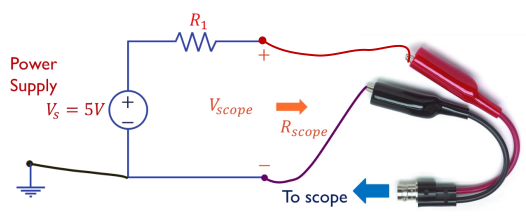
\includegraphics[width=0.5\textwidth]{oscilloscope resistance.png}
	\caption{Setup for measuring the Thevenin resistance of the oscilloscope. [1]}
	\label{fig:fig1}
\end{figure}

The setup in Figure \ref{fig:fig1} constructed.
\begin{figure}[H]
	\centering
	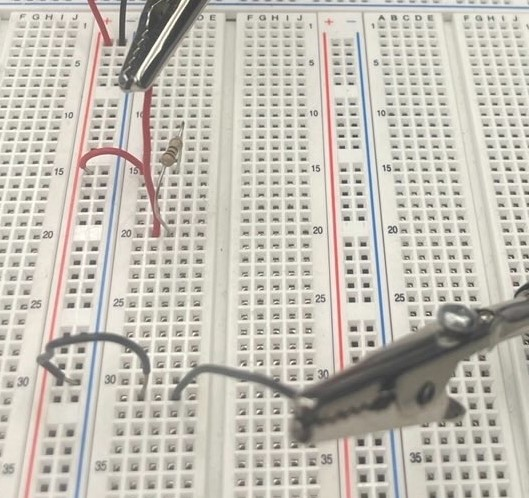
\includegraphics[width=0.5\textwidth]{circuit photo.jpg}
	\caption{Setup for measuring the Thevenin resistance of the oscilloscope.}
	\label{fig:fig2}
\end{figure}
The circuit found in Figure \ref{fig:fig2} was used to measure the Thevenin resistance of the 
oscilloscope. The resistance of the resistor used was $R = 0.969 \; M\Omega$. A voltage
of $V_{in} = 5.000 \; V$ was applied to the circuit. The voltage across the 
oscilloscope was measured to be $V_{osc} = 2.540 \; V$. This proves that the
the resistance of the oscilloscope is $R_{osc} = 0.999 \; M\Omega$.

\subsection*{Part 2}
The open circuit voltage of the signal generator was measured to 
be $V_{Th} = 1.000 \; V$. The 100 $\Omega$ resistor was connected to 
the signal generator in order to measure the Thevenin resistance. See
Figure \ref{fig:fig3} for the setup.

\begin{figure}[H]
	\centering
	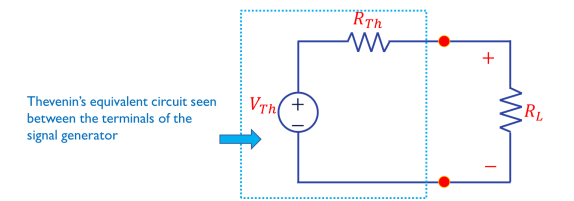
\includegraphics[width=0.75\textwidth]{signal generator.png}
	\caption{Measuring the Thevenin's equivalent circuit of the signal generator.}
	\label{fig:fig3}
\end{figure}
The actual resistance of the resistor was $R = 98.812 \; \Omega$. The 
voltage measured was 655.0 mV. This proves that the resistance of the 
signal generator is $R_{sig} = 52.04 \; \Omega$.
\begin{center}
\[
	V_L = V_{Th} \frac{R_L}{R_{Th} + R_L} \rightarrow 0.655 = 1 \frac{98.8}{R_{Th} + 98.8} \rightarrow R_{Th} = 52.04 \; \Omega
\]	
\end{center}
This comes very close to the marked value of $50 \; \Omega$ on 
the signal generator. A 47 $\Omega$ resistor was connected to the signal
generator. The actual resistance of $R_L = 46.771 \; \Omega$ The voltage
measured was 480 mV. 
\begin{center}
\[
	V_L = V_{Th} \frac{R_L}{R_{Th} + R_L} \rightarrow 0.480 = 1 \frac{46.771}{R_{Th} + 46.771} \rightarrow R_{Th} = 50.669 \; \Omega
\]	
\end{center}

This value is very close to the marked value of $50 \; \Omega$ on the 
signal generator and very close to the calculated value of $52.04 \; \Omega$.

\subsection*{Part 3}

\subsubsection*{Voltage Change Due to Oscilloscope Connection}

When an oscilloscope is connected to a signal generator, the input resistance of the oscilloscope and the output impedance of the signal generator form a voltage divider, which affects the voltage measured by the oscilloscope.


\begin{itemize}
	\item Let
	\begin{enumerate}
		\item \( V_{\text{open}} \) be the open-circuit voltage (without the oscilloscope).
		\item \( Z_{\text{out}} \) be the output impedance of the signal generator.
		\item \( R_{\text{in}} \) be the input resistance of the oscilloscope.
	\end{enumerate}
	\item Voltage Division: When the oscilloscope is connected, the voltage seen by the oscilloscope, \( V_{\text{load}} \), is:
	\[
	V_{\text{load}} = V_{\text{open}} \cdot \frac{R_{\text{in}}}{Z_{\text{out}} + R_{\text{in}}}
	\]
	\item Percentage Change in Voltage: The percentage change in voltage is given by:
	\[
	\% \text{Change} = \left( 1 - \frac{V_{\text{load}}}{V_{\text{open}}} \right) \times 100
	\]
	
	Substituting for \( V_{\text{load}} \):
	
	\[
	\% \text{Change} = \left( 1 - \frac{R_{\text{in}}}{Z_{\text{out}} + R_{\text{in}}} \right) \times 100
	\]
	
	Simplifying:
	
	\[
	\% \text{Change} = \left( \frac{Z_{\text{out}}}{Z_{\text{out}} + R_{\text{in}}} \right) \times 100
	\]
\end{itemize}

Thus, the percentage change in the open-circuit voltage when the oscilloscope is connected depends on the ratio of the signal generator's output impedance to the sum of the output impedance and the oscilloscope's input resistance.

\subsubsection*{Condition on Input Resistance for Minimal Effect}

To ensure that the oscilloscope or voltmeter does not affect the circuit's voltage by more than 1\%, the input resistance of the meter or oscilloscope should be significantly larger than the Thevenin equivalent resistance of the circuit.

\begin{itemize}
	\item Let
	\begin{enumerate}
		\item \( R_{\text{th}} \) be the Thevenin equivalent resistance of the circuit.
		\item \( R_{\text{in}} \) be the input resistance of the oscilloscope or voltmeter.
	\end{enumerate}
	\item Voltage Division: The condition for less than 1\% voltage change is:
	\[
   	\frac{R_{\text{in}}}{R_{\text{th}} + R_{\text{in}}} \geq 0.99
   	\]
	\item Rearranging:
	\[
	R_{\text{in}} \geq 99 \cdot R_{\text{th}}
	\]
\end{itemize}


Thus, the input resistance of the oscilloscope or voltmeter should be at least 100 times the Thevenin equivalent resistance to ensure a voltage change of less than 1\%.

\section{Discussion and Conclusion}

In this lab, the Thevenin equivalent models of both the oscilloscope 
and the signal generator were determined through practical experiments. 
By applying voltage division principles, we accurately measured the 
Thevenin resistance and open-circuit voltage for each device. For the 
oscilloscope, the measured Thevenin resistance of $R_{osc} = 0.999 \; 
M\Omega$ was consistent with expected values, demonstrating the high 
input resistance typically required to minimize loading effects on 
circuits under test. Similarly, the Thevenin resistance of the signal 
generator was calculated as $R_{sig} = 52.04 \; \Omega$, closely 
matching its rated output impedance.
\newline

These results emphasize the importance of understanding the interaction 
between measuring instruments and the circuits they probe. For instance, 
the effect of the oscilloscope’s input resistance on the measured 
voltage was demonstrated, showing how even a high-resistance instrument 
can alter the voltage reading if not properly accounted for. By ensuring 
that the input resistance of the measuring device is significantly 
larger (at least 100 times) than the circuit’s Thevenin resistance, 
voltage measurement errors can be minimized to less than 1\%.
\newline

The lab provided valuable insights into the practical use of Thevenin 
equivalents, highlighting how these simplified models enable more 
efficient circuit analysis. This knowledge is particularly relevant 
in designing and troubleshooting complex systems, where understanding 
the loading effects of various components and instruments is crucial 
for accurate measurements and overall system performance. 
\newline

Overall, the experiments successfully reinforced the theoretical 
concepts and provided a solid foundation for understanding how lab 
equipment interacts with circuits, ensuring accurate and reliable 
measurements in future engineering practice.


\section{References}
 [1] Dr. Iman Salama. “Lab 5 – Thevenin Equivalents of Lab Equipment” Northeastern University. 11 October 2024.

\end{document}
